\section{System}
The system we have designed consists of multiple parts,
one being a input device, another being a data processer, 
a third one being a communications service and the last one being a presenter.

\subsection{The Input Device}
Our motion tracking device(MTD) has been built in such a fashion that it resembles a wrist watch.
This form factor makes it rather compact.
Additionally a lot of people wear watches on a daily basis which makes the device of a recognizable morphology and barely noticeable for people accustomed to such devices.
The MTD contains a list of components, the most important are 6 Degrees of Freedom(6DoF) Sensor, Bluetooth and the Arduino microcontroller.

\begin{figure}[!h]
\centering
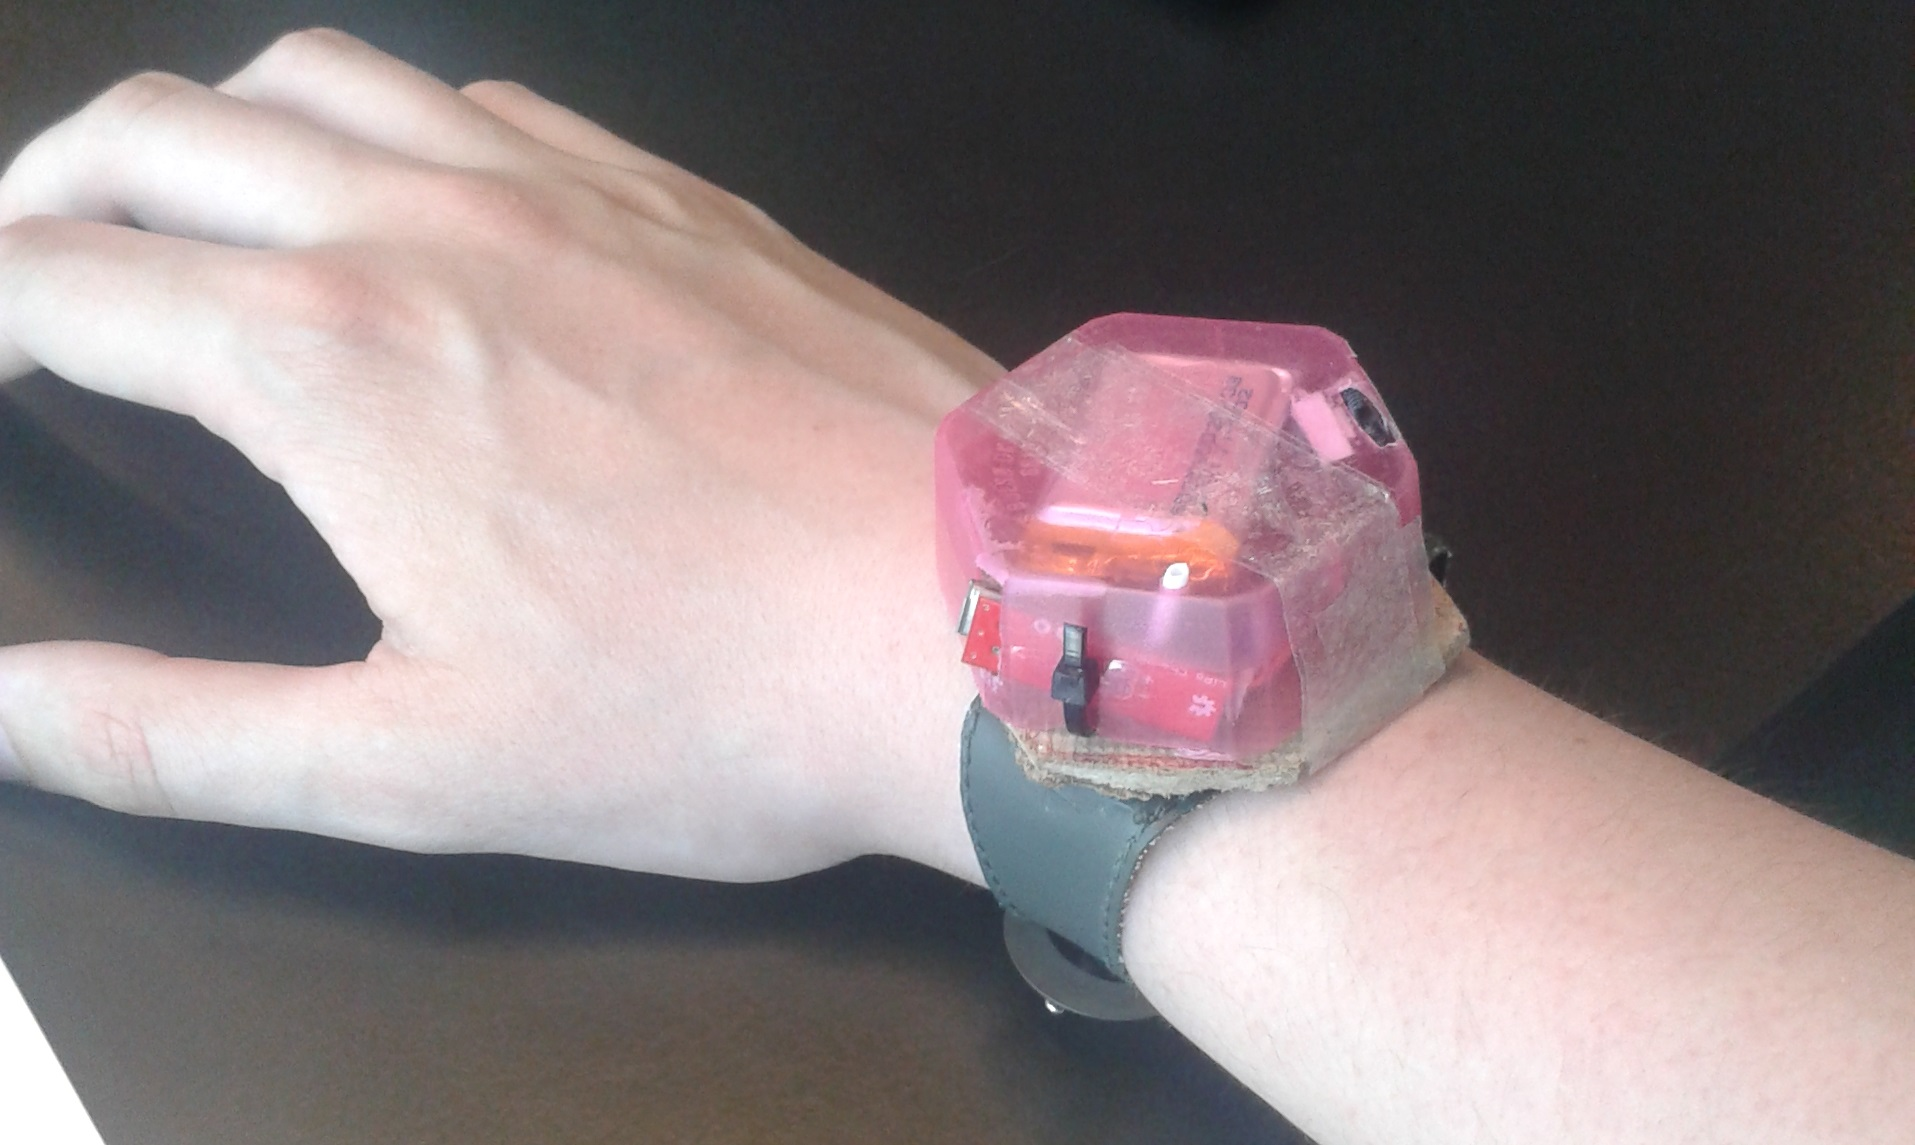
\includegraphics[width=1\columnwidth]{img/watch}
\caption{The input device.}
\label{fig:figure5}
\end{figure}

The \textbf{6DoF Sensor} is the heart of the device.
It is a board which contains an accelerometer and a gyroscope.
This means that it is possible to measure movement and rotation of the wrist of anyone wearing the device.
The sensor produces a set of 6 values: 3 for acceleration and 3 for rotation, each representing information on the axes of the coordinate system.
The input received from the 6DoF sensor is then propagated to the \textbf{arduino microcontroller}.
The arduino prepares the raw  values into JSON data. The JSON is then sent using the bluetooth device.

\begin{figure}[!h]
\centering
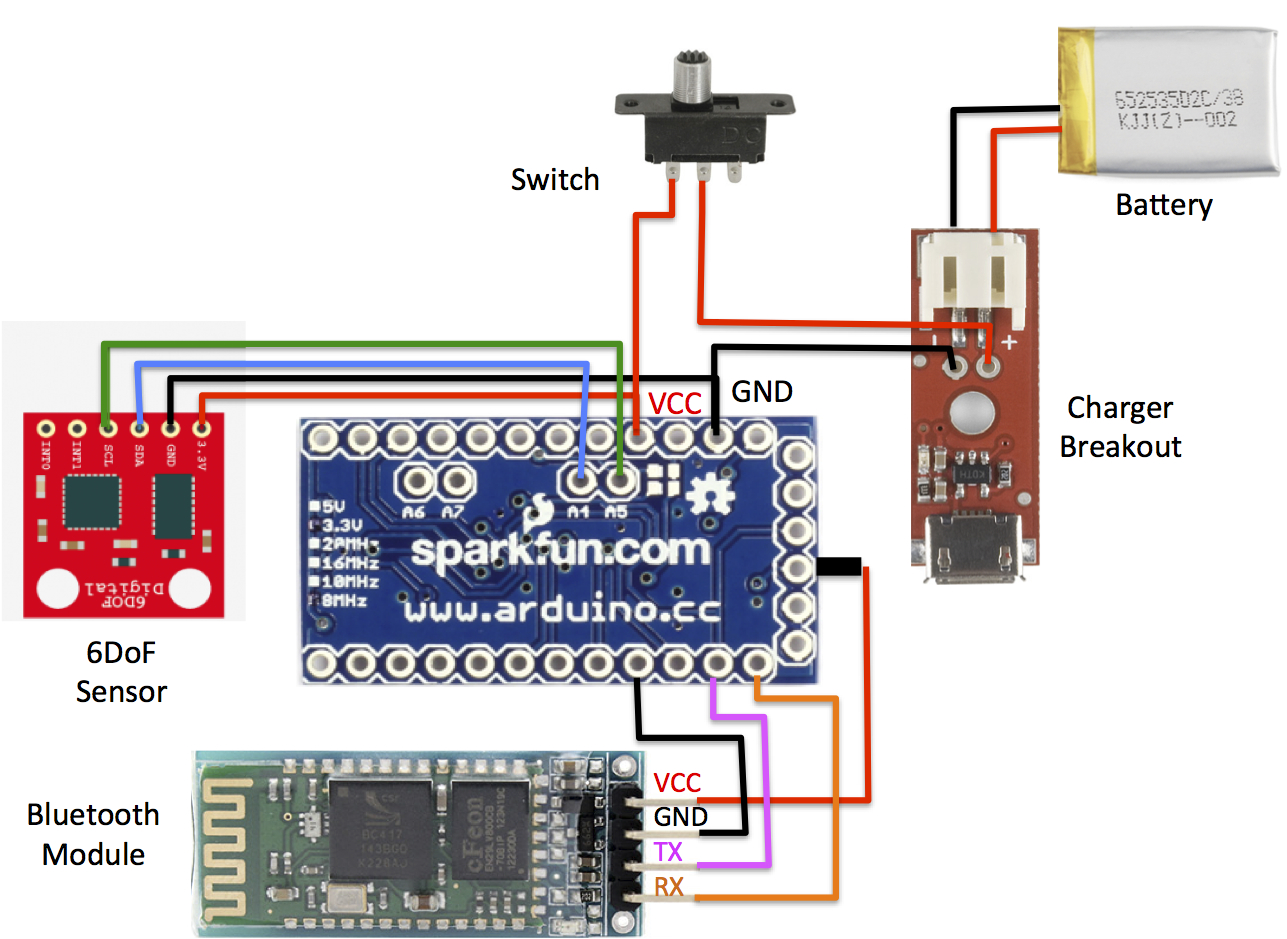
\includegraphics[width=1\columnwidth]{img/device_schematic}
\caption{This schematic shows the circuitry on the device.}
\label{fig:figure1}
\end{figure}

\subsection{Weka Gesture Recognition System}
Since the input device we have built is quite lightweight, data processing needs to be done elsewhere.

This provided us with the challenge of transferring data from one bluetooth capable device to another.
All the processing and preprocessing of the device's data is performed on a desktop application on a 
computer connected to the device via bluetooth.

One of the biggest challenges was to find and integrate Java libraries which would allow the system to establish such a  
connection to the MTD.

Data exchange is crucial to be able to process it in the desktop application and recognize patterns.
Processing covers the steps of preprocessing and classifying; once these steps have been completed a gesture is hopefully recognized.


%This component of the system is responsible for the preprocessing of the data and the gesture recognition. 
Every time a gesture is recognized by the system, an identifier of the gesture is sent from the desktop application to the webservice where it will be available for its final consumer: the android application.


For further technical details about the challenges encountered please refer to the System implementation section and the Technical challenges section.

\subsection{Android Application}
The android system is a quite limited system.
It is able to display an image as seen on figure \ref{fig:android1}.

It provides the user with the possibility of panning and zooming a given image.
When the user zooms all the way out, panning provides additional functionality such as
being able to swap images from a set of loaded images as seen on figure \ref{fig:android2}.

\begin{figure}[!h]
\centering
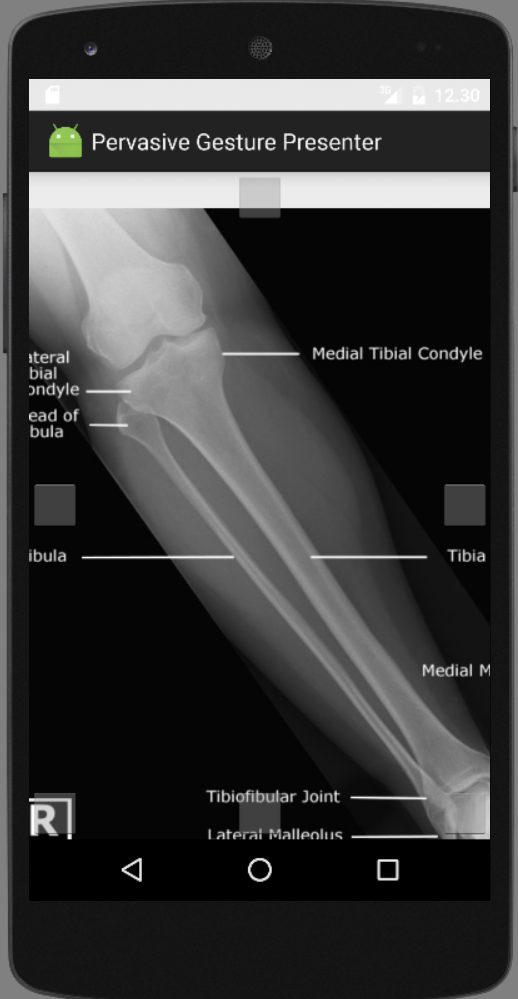
\includegraphics[width=0.4\columnwidth]{img/android_main}
\caption{Interface of the android image presenter}
\label{fig:android1}
\end{figure}

\begin{figure}[!h]
\centering
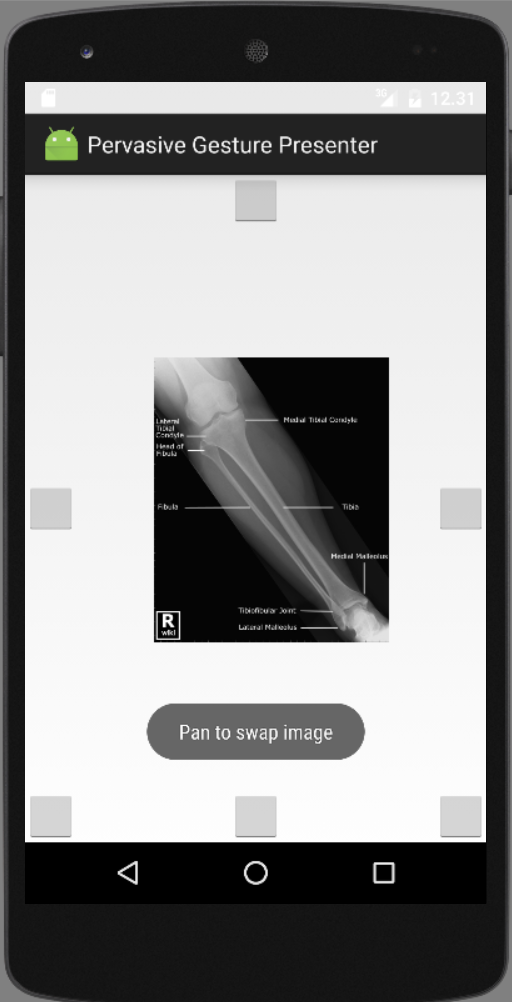
\includegraphics[width=0.4\columnwidth]{img/android_zoom_pan}
\caption{ Image of pan to swap image functionality.}
\label{fig:android2}
\end{figure}

\subsection{Webservice}
The communication between the Weka Gesture Recognition System and the Android Application is done by a simple webservice.
It provides GET, POST and DELETE requests which manipulate a queue.

GET pops all the queued gesture recognitions, 
POST pushes a new one to the service and DELETE clears the queue.

\begin{figure}[!h]
\centering
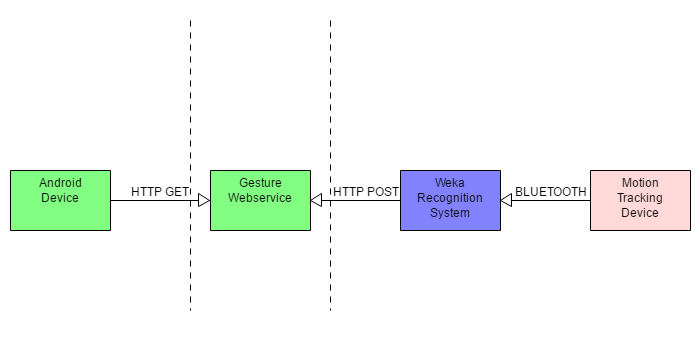
\includegraphics[width=0.9\columnwidth]{img/system_diagram}
\caption{This schematic shows the system interactions.}
\label{fig:sys}
\end{figure}